\documentclass[border=12pt]{standalone}
\usepackage{tikz}
\usetikzlibrary{arrows.meta,positioning,fit,calc}

\definecolor{encfill}{RGB}{220,235,250}
\definecolor{encborder}{RGB}{60,110,170}
\definecolor{decfill}{RGB}{255,235,220}
\definecolor{decborder}{RGB}{180,90,40}
\definecolor{attnfill}{RGB}{230,220,250}
\definecolor{attnborder}{RGB}{100,70,160}
\definecolor{fffill}{RGB}{220,245,230}
\definecolor{ffborder}{RGB}{50,140,90}
\definecolor{normfill}{RGB}{250,250,230}
\definecolor{normborder}{RGB}{140,130,60}
\definecolor{embfill}{RGB}{240,240,245}
\definecolor{embborder}{RGB}{90,90,110}
\definecolor{outfill}{RGB}{255,245,210}
\definecolor{outborder}{RGB}{160,120,40}
\definecolor{arrowcol}{RGB}{50,50,50}
\definecolor{stackbg}{RGB}{248,250,252}
\definecolor{crosscol}{RGB}{160,60,60}

\begin{document}
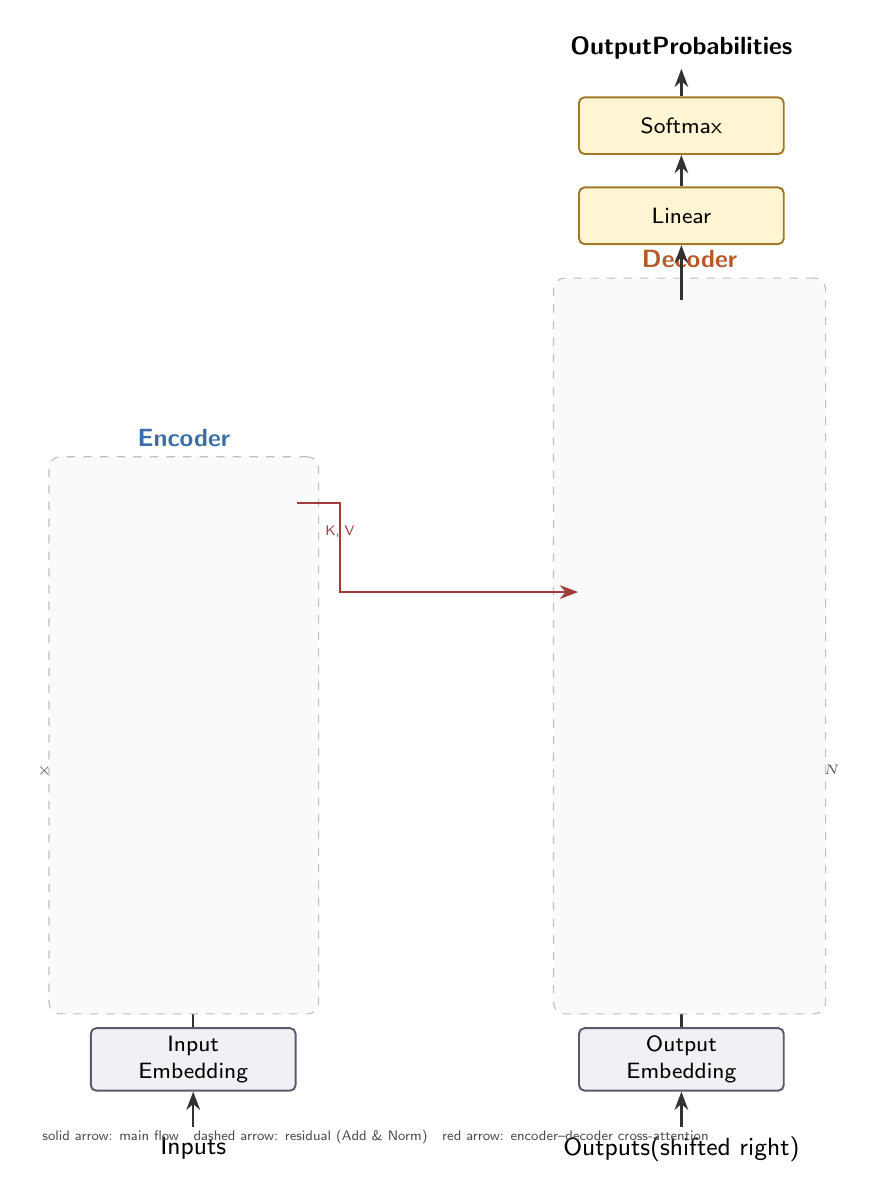
\begin{tikzpicture}[
  >=Stealth,
  font=\sffamily\footnotesize,
  block/.style={
    draw,
    rounded corners=2pt,
    align=center,
    minimum width=2.6cm,
    minimum height=0.72cm,
    line width=0.7pt,
    inner sep=3pt
  },
  enc/.style={block, fill=encfill, draw=encborder},
  dec/.style={block, fill=decfill, draw=decborder},
  attn/.style={block, fill=attnfill, draw=attnborder},
  ff/.style={block, fill=fffill, draw=ffborder},
  norm/.style={block, fill=normfill, draw=normborder, minimum height=0.58cm},
  emb/.style={block, fill=embfill, draw=embborder},
  outblk/.style={block, fill=outfill, draw=outborder},
  flow/.style={->, thick, color=arrowcol},
  residual/.style={->, thick, color=encborder, dashed},
  cross/.style={->, thick, color=crosscol},
  stackbox/.style={
    draw=gray!50,
    dashed,
    rounded corners=4pt,
    fill=stackbg,
    inner sep=8pt
  },
  lbl/.style={font=\sffamily\tiny, text=gray!70!black}
]

% ========== Encoder (left) ==========
\node[emb] (enc-in) at (0,0) {Input\\Embedding};
\node[emb, above=0.45cm of enc-in] (enc-pe) {Positional\\Encoding};
\node[norm, above=0.55cm of enc-pe] (enc-an1) {Add \& Norm};
\node[attn, above=0.45cm of enc-an1] (enc-mha) {Multi-Head\\Attention};
\node[norm, above=0.45cm of enc-mha] (enc-an2) {Add \& Norm};
\node[ff, above=0.45cm of enc-an2] (enc-ff) {Feed\\Forward};
\node[norm, above=0.45cm of enc-ff] (enc-an3) {Add \& Norm};

% Encoder residual bypasses
\coordinate (enc-res1-l) at ($(enc-pe.north)+(-1.55,0)$);
\coordinate (enc-res1-t) at ($(enc-an1.west)+(-0.05,0)$);
\coordinate (enc-res2-l) at ($(enc-an1.north)+(-1.55,0)$);
\coordinate (enc-res2-t) at ($(enc-an2.west)+(-0.05,0)$);
\coordinate (enc-res3-l) at ($(enc-an2.north)+(-1.55,0)$);
\coordinate (enc-res3-t) at ($(enc-an3.west)+(-0.05,0)$);

% Encoder vertical flow
\draw[flow] (enc-in) -- (enc-pe);
\draw[flow] (enc-pe) -- (enc-an1);
\draw[flow] (enc-an1) -- (enc-mha);
\draw[flow] (enc-mha) -- (enc-an2);
\draw[flow] (enc-an2) -- (enc-ff);
\draw[flow] (enc-ff) -- (enc-an3);

% Encoder residuals (skip connections into Add & Norm)
\draw[residual] (enc-pe.north) -- ++(0,0.12) -| (enc-res1-l) |- (enc-an1.west);
\draw[residual] (enc-an1.north) -- ++(0,0.12) -| (enc-res2-l) |- (enc-an2.west);
\draw[residual] (enc-an2.north) -- ++(0,0.12) -| (enc-res3-l) |- (enc-an3.west);

% Encoder Nx label
\node[lbl, left=0.15cm of enc-mha] {$\times N$};

\node[stackbox, fit=(enc-pe)(enc-mha)(enc-ff)(enc-an3)(enc-res1-l)(enc-res3-l),
  label={[font=\sffamily\small\bfseries, text=encborder]above:Encoder}] (enc-stack) {};

% ========== Decoder (right) ==========
\node[emb] (dec-in) at (6.2,0) {Output\\Embedding};
\node[emb, above=0.45cm of dec-in] (dec-pe) {Positional\\Encoding};
\node[norm, above=0.55cm of dec-pe] (dec-an1) {Add \& Norm};
\node[attn, above=0.45cm of dec-an1] (dec-mmha) {Masked Multi-Head\\Attention};
\node[norm, above=0.45cm of dec-mmha] (dec-an2) {Add \& Norm};
\node[attn, above=0.45cm of dec-an2] (dec-cross) {Multi-Head\\Cross-Attention};
\node[norm, above=0.45cm of dec-cross] (dec-an3) {Add \& Norm};
\node[ff, above=0.45cm of dec-an3] (dec-ff) {Feed\\Forward};
\node[norm, above=0.45cm of dec-ff] (dec-an4) {Add \& Norm};

% Decoder vertical flow
\draw[flow] (dec-in) -- (dec-pe);
\draw[flow] (dec-pe) -- (dec-an1);
\draw[flow] (dec-an1) -- (dec-mmha);
\draw[flow] (dec-mmha) -- (dec-an2);
\draw[flow] (dec-an2) -- (dec-cross);
\draw[flow] (dec-cross) -- (dec-an3);
\draw[flow] (dec-an3) -- (dec-ff);
\draw[flow] (dec-ff) -- (dec-an4);

% Decoder residuals
\coordinate (dec-res1-r) at ($(dec-pe.north)+(1.55,0)$);
\coordinate (dec-res2-r) at ($(dec-an1.north)+(1.55,0)$);
\coordinate (dec-res3-r) at ($(dec-an2.north)+(1.55,0)$);
\coordinate (dec-res4-r) at ($(dec-an3.north)+(1.55,0)$);

\draw[residual] (dec-pe.north) -- ++(0,0.12) -| (dec-res1-r) |- (dec-an1.east);
\draw[residual] (dec-an1.north) -- ++(0,0.12) -| (dec-res2-r) |- (dec-an2.east);
\draw[residual] (dec-an2.north) -- ++(0,0.12) -| (dec-res3-r) |- (dec-an3.east);
\draw[residual] (dec-an3.north) -- ++(0,0.12) -| (dec-res4-r) |- (dec-an4.east);

\node[lbl, right=0.15cm of dec-mmha] {$\times N$};

\node[stackbox, fit=(dec-pe)(dec-mmha)(dec-cross)(dec-ff)(dec-an4)(dec-res1-r)(dec-res4-r),
  label={[font=\sffamily\small\bfseries, text=decborder]above:Decoder}] (dec-stack) {};

% ========== Output head ==========
\node[outblk, above=0.7cm of dec-an4] (linear) {Linear};
\node[outblk, above=0.4cm of linear] (softmax) {Softmax};
\node[above=0.35cm of softmax, font=\sffamily\small\bfseries] (probs) {Output\\Probabilities};

\draw[flow] (dec-an4) -- (linear);
\draw[flow] (linear) -- (softmax);
\draw[flow] (softmax) -- (probs);

% ========== Cross connection: Encoder → Decoder Cross-Attention ==========
\draw[cross] (enc-an3.east) -- ++(0.55,0) |- (dec-cross.west)
  node[pos=0.25, above, font=\sffamily\tiny, text=crosscol] {K, V};

% ========== Bottom inputs ==========
\node[below=0.45cm of enc-in, font=\sffamily\small] (inputs) {Inputs};
\node[below=0.45cm of dec-in, font=\sffamily\small] (outputs) {Outputs\\(shifted right)};
\draw[flow] (inputs) -- (enc-in);
\draw[flow] (outputs) -- (dec-in);

% ========== Legend ==========
\node[anchor=north west, font=\sffamily\tiny, align=left, text=gray!60!black]
  at ($(enc-stack.south west)+(-0.2,-1.35)$) {
  solid arrow: main flow\quad
  dashed arrow: residual (Add \& Norm)\quad
  red arrow: encoder--decoder cross-attention
};

\end{tikzpicture}
\end{document}
